% !TeX root = ../main.tex

\subsection*{(Kernel) PCA}

Our known approch is the principle component analysis (PCA).

\begin{figure}[H]
	\centering
	\begin{minipage}[b]{0.6\textwidth}
		\begin{itemize}
			\item eigen-decomposition of covariance matrix $\Sigma$
			\item reduce dimensions by dropping eigenvectors with smaller eigenvalues
			\item transform data to lower dimensional space by multiplying the matrix of eigenvectors with the data matrix \[X_{low} = X_{high} \cdot W_{low}\] where $W_{low}$ is a matrix of the wanted number of eigenvectors in its columns
		\end{itemize}
	\end{minipage}
	\begin{minipage}[b]{0.3\textwidth}
		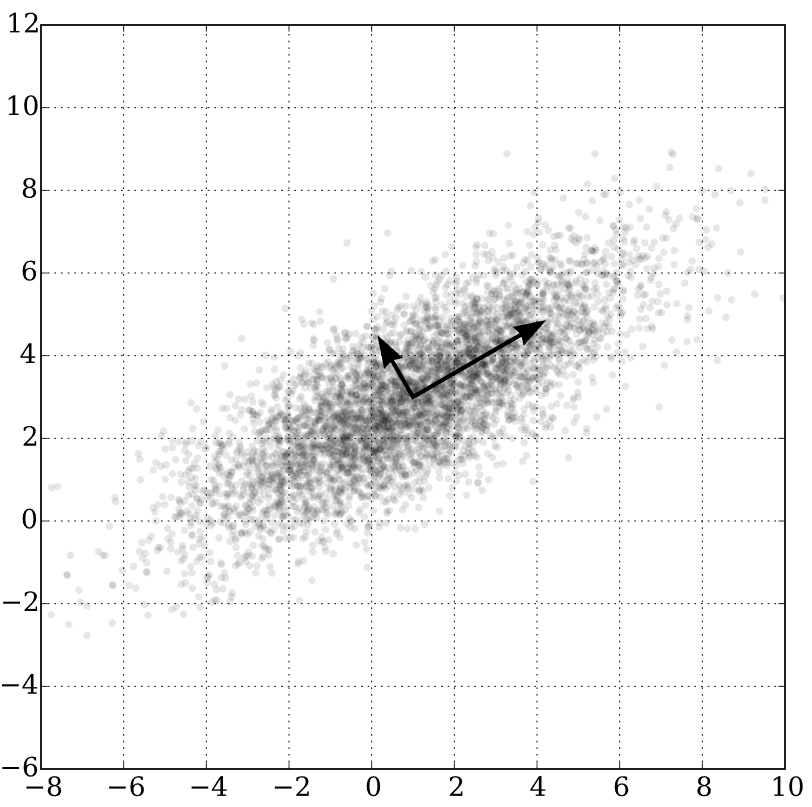
\includegraphics[width=\textwidth]{pca_wiki}
	\end{minipage}
\end{figure}

Orthogonal basis that is aligned with the ``maximum spread'' (w.r.t. the covariance) of the data. It is a global unsupervised method\footnote{Operating on all data points, no labels, find one global optimal solution}. PCA is a linear method, which is problematic when we want a non-linear mapping of our data.

\begin{equation*}
    \sum_{i}^{N} (\vec{n}^T \vec{x_i}) (\vec{n}^T \vec{x_i}) + \lambda (\vec{n}^T \vec{n} - 1)
\end{equation*}

\begin{figure}[H]
	\centering
	\begin{minipage}[b]{0.45\textwidth}
		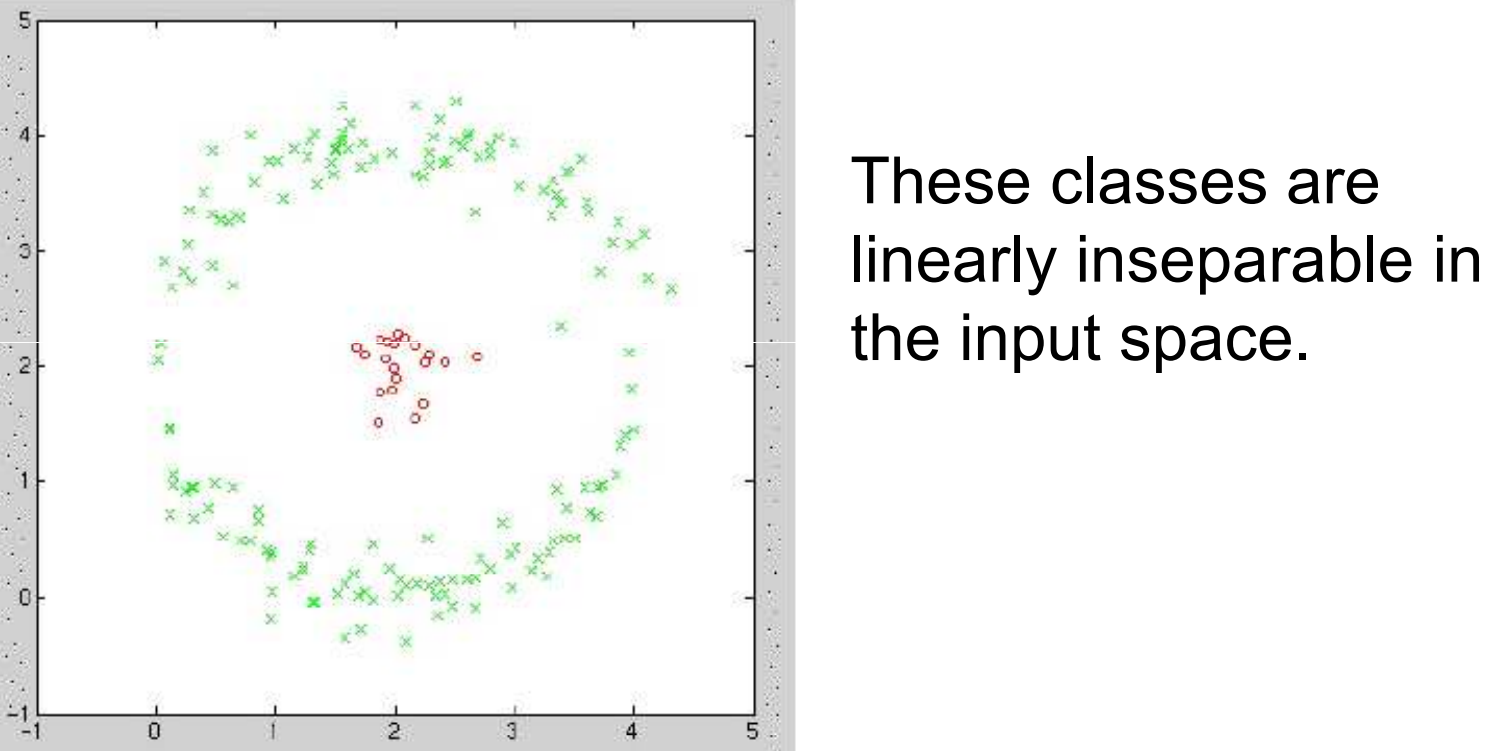
\includegraphics[width=\textwidth]{kpca1}
	\end{minipage}
	\begin{minipage}[b]{0.45\textwidth}
		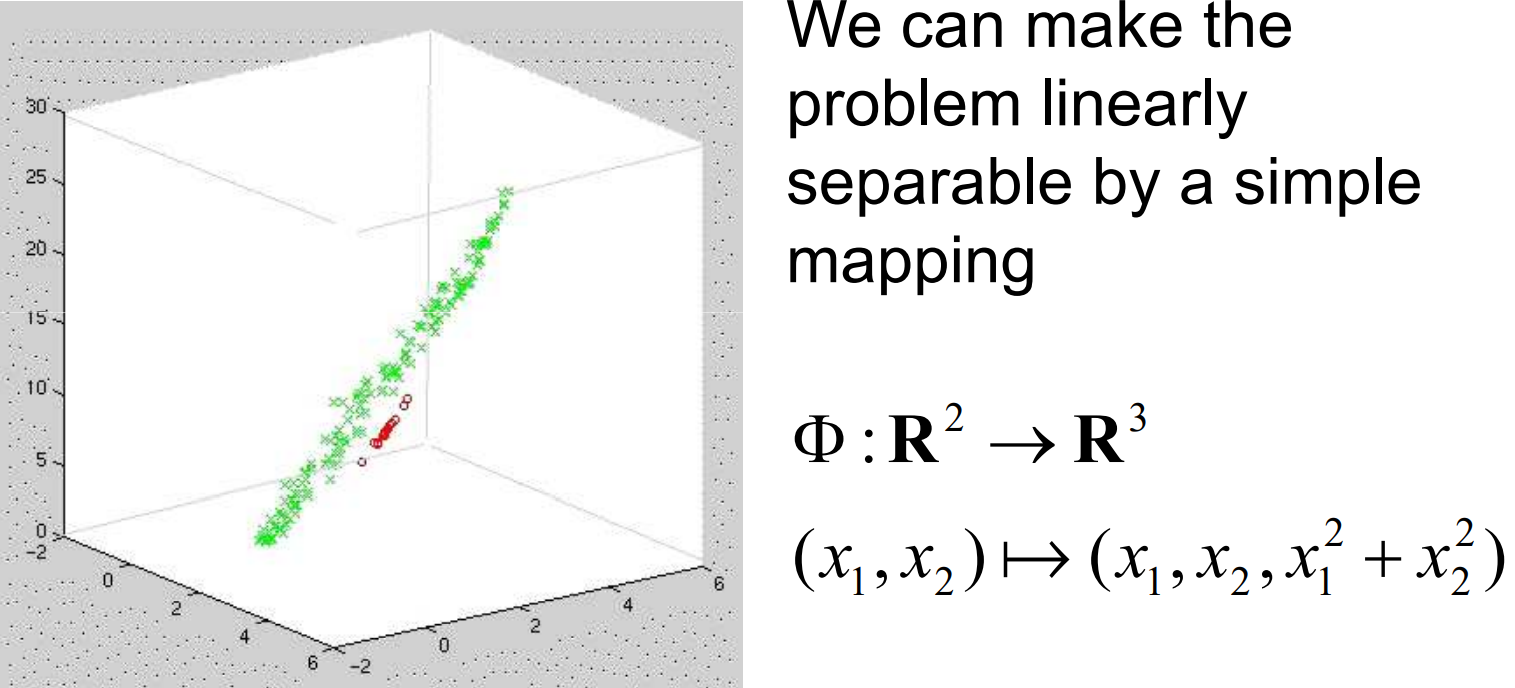
\includegraphics[width=\textwidth]{kpca2}
	\end{minipage}
\end{figure}

The Kernel PCA performs a non-linear mapping of the data, then perform a standard (linear) PCA on the result. With the kernel-trick we can do that in one step. The Objective function: (the non-linear mapping is part of $\phi$)

% TODO: better explanaition

\begin{equation*}
    \delta = \sum_{i,j=1}^{N} (\phi(\vec{x_i}) - \phi(\vec{x_j}))^T (\phi(\vec{x_i}) - \phi(\vec{x_j})) + \lambda (\phi^T\phi-1)
\end{equation*}

Some offsprings of the Kernel PCA idea are:
\begin{enumerate}
    \item Perform some preprocessing / mapping that operates non-linearly
    \item The dimensionality reduction itself is an operation that operates linearly.
\end{enumerate}
